\begin{refsection}
\chapter{The interplay of environmental conditions, parameter sensitivity and structural sensitivity in predictions of species coexistence} % Main chapter title
\label{Bayesian_competition}

\noindent Alba Cervantes-Loreto\textsuperscript{1}, Abigail Pastore \textsuperscript{2}, Christopher R.P.\ Brown\textsuperscript{1},Michelle L.\ Maraffini\textsuperscript{1},Clement Aldeber\textsuperscript{3},Clement Aldeber\textsuperscript{3},Margaret M.\ Mayfield\textsuperscript{2},Stouffer Daniel B.\textsuperscript{1}

\begin{enumerate}
    \item Centre for Integrative Ecology, School of Biological Sciences, University of Canterbury, New Zealand
    \item School of Biological Sciences, University of Queensland, Brisbane, Australia
    \item Aix Marseille Univ., Université de Toulon,  Marseille, France
\end{enumerate}

\end{refsection}
\section*{Abstract}


Predicting the outcome of competitive interactions among species that share resources is central to our current understanding of diversity maintenance. However, we have little information about how robust are predictions of species coexistence. This limitation is partly because several sources of uncertainty are often ignored when making predictions. Here, we introduce a mathematical and statistical framework to simultaneously explore how different models, environmental contexts and parameter uncertainty change the probability of predicting species coexistence.  Using a set of pairwise competition experiments of annual plants, we provide direct evidence that seemingly subtle differences between models led to predictions of both coexistence and competitive exclusion based around the exact same experimental data. We also show that the effects of environmental context-dependency and parameter uncertainty on predictions of species coexistence are not independent of the model formulation used to describe species dynamics. Our work suggests that predictions of species coexistence and extrapolations made from them are particularly vulnerable to change due to the three sources of uncertainty we studied.

\section*{Introduction}


The effects species have on one another are the result of multiple processes that often act simultaneously. In the case of competition between plants, examples include the depletion of local resources in the soil \citep{dybzinski2007resource, craine2013mechanisms},  visits from shared pollinators \citep{lanuza_opposing_2018}, or the frequency and intensity of disturbance events \citep{pickett1980non, villarreal2009species}. Notwithstanding their importance, fully including all such phenomena in the study of plant dynamics is often impractical. Hence, it is more straightforward to treat these processes implicitly and model the relationship between interacting species phenomenologically, for example by fitting models that describe how the densities of intraspecific and interspecific neighbors change plant fitness and growth \citep{case1999illustrated, adler2018competition}.


Despite their ``necessary incompleteness'', phenomenological models can accurately reproduce the observed data in various natural systems and contexts \citep{bolker_ecological_2008}. Perhaps more importantly, they are useful tools with which to make predictions that extend beyond the phenomena they describe. Such predictions are possible because of the implicit assumption that models that reproduce the observed data faithfully also capture how the studied system operates \citep{marquet2015importance}. For example, models that describe the effects neighboring plants have on each other can be used to make quantitative predictions about changes of biomass in the system \citep{godoy2020excess, lai2020role} or qualitative predictions such as whether or not co-occurring plant species can coexist \citep{levine2009importance, zepeda2019fluctuation}.

% some references you might be looking for in terms of "...operates" above are:
% Klir, G. J., 1985. Architecture of Systems Problem Solving. Plenum Press, New York, NY, USA.
% Zeigler, B. P., Praehofer, H., and Kim, T., 2000. Theory of Modeling and Simulation. Academic Press, San Diego, CA, USA.
% Marquet, P. A., Allen, A. P., Brown, J. H., Dunne, J. A., Enquist, B. J., Gillooly, J. F., Gowaty, P. A., Harte, J., Hubbell, S. P., Okie, J. G., Ostling, A., Ritchie, M., Storch, D., and West, G. B. 2015. On the importance of first principles in ecological theory development. BioScience 65:342–343.

The practicality of phenomenological models of plant competition, however, is a double-edged sword. Indeed, predictions made with them are subject to uncertainty arising from many distinct sources. One of these is environmental context dependency, or the extent to which the outcomes of species interactions change as a function of the abiotic conditions species experience \citep{chamberlain_how_2014}. Many studies have documented how the sign and magnitude of species interactions change with environmental conditions, such as interspecific interactions between plants switching from competitive to facilitative in harsh environments \citep{callaway_positive_2002, maestre2005change, brooker2008facilitation,maestre2009refining}, changes to the identity of the competitive superior plant species as abiotic conditions change \citep{poorter1986growth, dybzinski2007resource}, or variations in interaction strength between plants along environmental gradients \citep{bimler_accurate_2018, villarreal2009species, lanuza_opposing_2018}. Extrapolations from phenomenological models of plant competition can therefore be highly specific to the set of conditions under which models were parameterized \citep{bimler_accurate_2018}.


Model-based predictions are also subject to two forms of uncertainty that arise from the use of models themselves: parameter sensitivity and structural sensitivity. Parameter sensitivity refers to the sensitivity of model outputs to variation in parameter values \citep{flora_structural_2011}, and exploring it constitutes a routine analysis in the domain of the biological sciences \citep{jorgensen2001fundamentals}. On the other hand, structural sensitivity characterizes how  mathematical expressions that have similar phenomenological behavior can produce qualitatively different outcomes \citep{flora_structural_2011,myerscough1996stability,aldebert2018community}. Parameter and structural sensitivity are often intertwined \citep{wood1999super}, and both have been shown to drastically change model predictions in a vast array of biological systems \citep{flora_structural_2011, wood1999super, poggiale2010far, fussmann2005community,  aldebert2018community}.

The interplay between environmental context dependency, parameter sensitivity, and structural sensitivity is rarely explored simultaneously, and to the best of our knowledge  has never been explicitly explored in the case of models of density dependence in plant performance. In this study, we therefore aim to understand how these three sources of uncertainty change predictions of a widely studied and vastly important ecological process: species coexistence. We focused our analysis on annual plants, which is a common natural system used to study species coexistence \citep{mayfield2017higher, godoy_phenology_2014,levine2009importance, zepeda2019fluctuation}. We assessed the empirical relevance of the three different sources of uncertainty by making coexistence predictions based around data from a competition experiment between two annual plants conducted in two contrasting abiotic conditions. Our analyses provide evidence that uncertainty can radically change predictions made from a simple competition experiment, and highlights the importance of incorporating uncertainty from different sources in predictions made with phenomenological models.

\section*{Methods}

We will first provide a mathematical description of how to make and interpret coexistence predictions made with a single phenomenological model of two species of annual plants growing in proximity to each other. We then expand our framework to introduce an alternative phenomenological model of plant density dependence, and show how our framework can be used to make predictions using a different model per species. Second, we describe how to use a Bayesian framework to parameterize the  aforementioned  phenomenological models  to data from a set of competition experiments between two annual plants growing in two contrasting abiotic conditions. Finally, we describe how we simultaneously explored structural sensitivity, parameter sensitivity, and environmental context dependency to make predictions of species coexistence.


\subsection*{Model-based predictions of species coexistence }

We used the Cohen model \citep{cohen1966optimizing,watkinson_density-dependence_1980} to describe annual-plant population dynamics and as the starting point for our model-based predictions of species coexistence. This model predicts the number of seeds $N_{i,t+1}$ from species $i$ in year $t+1$ with:
\begin{equation}
\label{annual_plant}
    N_{i,t+1}= (1-g_i)s_{i} N_{i,t}  + g_{i} N_{i,t}F_{i,t}\,,
\end{equation}
which is a function of prior number of seeds in the soil ($N_{i,t}$) that survive that year in the seed bank (as weighted by $s_{i}$, the fraction of non-germinating seeds that survive in the soil), and the seeds that germinate (described by $g_i$) multiplied by the number of viable seeds produced per seed germinated, often called their realized fecundity ($F_{i,t}$). The realized fecundity of species \textit{i} can be accurately described by many different phenomenological forms \citep{law_response-surface_1987, godwin2020empiricist}. Note that the phenomenological descriptions of $F_{i,t}$ generally try to capture the density dependence of plant performance on the number of conspecific and heterospecific neighbors, but do not necessarily imply a hypothesis about the mechanisms underpinning this density dependence.

As an example, $F_{i,t}$ can be given by the Beverton--Holt model \citep{beverton1954notes}, which in a two-species context equals:
 \begin{equation}
 \label{Beverton-Holt}
    F_{i,t} = \frac{\lambda_{i}}{1 + \alpha_{ii}g_{i}N_{i,t} + \alpha_{ij}g_{j}N_{j,t}}\,.
\end{equation}
In this model, the per germinant fecundity of species \textit{i} in the absence of competition is described by the parameter $\lambda_{i}$, while the numbers of germinants of species $i$ and $j$ in year $t$ are given by $g_{i}N_{i,t}$ and $g_{j}N_{j,t}$, respectively. The density-dependent effects are captured by the interaction coefficients $\alpha_{ii}$ and $\alpha_{ij}$, which describe the interaction strength of conspecifics and heterospecifics, respectively. The Beverton--Holt model is a commonly used phenomenological model to make coexistence predictions and can be easily parameterized with empirical observations of annual plants growing in proximity to each other \citep{godoy_phenology_2014, godoy_phylogenetic_2014, levine2009importance}.

\subsubsection*{Coexistence predictions}

From the population dynamics that result from using Eqn.~\ref{annual_plant} and estimates of the relevant parameters of Eqns.~\ref{annual_plant} and ~\ref{Beverton-Holt},  it is possible to predict if a pair of species can coexist. Multiple approaches exist to predict species coexistence \citep{chesson_general_2000, chesson_updates_2018, barabas_chessons_2018, saavedra2017structural, letten_linking_2017}. One of them is to directly evaluate, given the competitive constraints each species experiences, if the set of species intrinsic growth rates is feasible \citep[i.e., if there exists an equilibrium point under which both species have positive abundances;][]{rohr_structural_2014, saavedra2017structural}. To do so, it is necessary to derive the equations determining the equilibrium density for each species, which for species $i$ is found at:

\begin{equation}
\label{equilbrium}
  \frac{N_{i,t+1}}{N_{i,t}}  = (1-g_{i})s_{i} + \frac{g_{i}\lambda_{i}}{1 + \alpha_{ii}g_{j}N_{i}^{*} + \alpha_{ij}g_{j}N_{j}^{*}}  = 1 .
\end{equation}

This equilibrium condition can be arranged to provide a linear equation in terms of seed densities:
\begin{equation}
\label{bh_equilibrium}
    -1 + \left( \frac{g_{i}\lambda_{i}}{1-(1-g_{i})s_{i}} \right) = \alpha_{ii}g_{i}N_{i}^{*} + \alpha_{ij}g_{j}N_{j}^{*}.
\end{equation}
For reasons that will hopefully become clear later, Eqn.~\ref{bh_equilibrium} can be rewritten as:
\begin{equation}
  \label{growth_competition}
  r_{i} = \alpha_{ii}g_{i}N_{i}^{*} + \alpha_{ij}g_{j}N_{j}^{*},
\end{equation}
where $r_{i}$ is the intrinsic growth rate of  species $i$. Note that $r_{i}$ is a composite parameter that depends on the values of $s_{i}$, $g_{i}$, and $\lambda_{i}$. Equivalent expressions for species $j$ can be derived from its equilibrium condition. The combined two-species equilibrium condition is:
\begin{equation}
\begin{bmatrix}
r_{i} \\
r_{j}
\end{bmatrix} =
\begin{bmatrix}
\alpha_{ii} &  \alpha_{ij} \\
\alpha_{ji} & \alpha_{jj}
\end{bmatrix}
\begin{bmatrix}
g_{i}N_{i}^{*}\\ g_{j}N_{j}^{*}
\end{bmatrix} \,.
\label{twosp}
\end{equation}
Given estimates of $r_{i}$, $r_{j}$, and the matrix of competition coefficients, $A$, predicted species densities at equilibrium can be solved for by rearranging Eqn.~\ref{twosp} to:
\begin{equation}
\begin{bmatrix}
g_{i}N_{i}^{*}\\
g_{j}N_{j}^{*}
\end{bmatrix} =
A^{-1}
\begin{bmatrix}
r_{i}\\ r_{j}
\end{bmatrix} \,.
\label{abundances}
\end{equation}

When predicted equilibrium abundances for both species are positive, then the model-based prediction is that they can coexist \citep{rohr_structural_2014,saavedra2017structural}. In contrast, if one of the predicted equilibrium abundances is less or equal to zero, then model-based predictions is that one of the species is competitively excluding the other. Finally, if both predicted equilibrium abundances are less or equal to zero, then none of the species can persist in the system according to the model used to make predictions.


\subsubsection{Biologically-constrained feasibility domain}

In practice, it is useful not only to determine if fixed values of $r_{i}$ and $r_{j}$ allow species to coexist, but to explore the full set of  values of species growth rates that are compatible with species coexistence. This approach is often referred to as \textit{the structural approach}, and is easily applicable to annual-plant dynamics \citep{saavedra2017structural}. The parameter space where both species can have positive abundances at equilibrium,  given the constraints imposed through the competition matrix, is called the feasibility domain \citep{rohr_structural_2014, saavedra2017structural, song_guideline_2018, song_towards_2020}. Biologically, a large feasibility domain  means that competition is lax, and species can grow at different rates without excluding each other. In contrast, a small feasibility domain means that competitive constraints are harsh, and only a handful of growth rates allow their coexistence.

Importantly, locations in the growth-rate parameter space carry direct biological interpretations with them. Consider, for example, a growth-rate vector $r$ that allows for positive equilibrium abundances $N$. Any proportional vector $xr$ will also produce $xN$ as a solution to Eqn.~\ref{abundances}. However, it is reasonable to assume that there exists an upper limit to species' abundances in nature (i.e., we do not expect species to achieve infinite abundances). If a growth-rate vector leads to predicted abundances beyond a particular species' observable limit, we argue it should not be considered biologically feasible. The imposition of an abundance constraint such as this one will tend to create an upper bound on the growth rates that define the feasibility domain.

In addition, the Beverton--Holt model implicitly imposes further biological constraints on the values species growth rates can take. Recall that a species' composite growth rate, $r_{i}$, is a product of three biologically-meaningful parameters. Those parameters have bounds themselves and when combined together they can further impact the values species' composite growth rates can take. Specifically, $s_{i}$ and $g_{i}$ are proportions and can only have values between zero and one, while the per germinant fecundity in the absence of competition $\lambda_{i}$ can only have positive values. By assuming density dependence for a given species follows the Beverton--Holt model, these parameter constraints together imply that growth rates $r_i < -1$ are not biologically feasible. Any value of $r_{i} < -1$ corresponds to $\left( \frac{g_{i}\lambda_{i}}{1-(1-g_{i})s_{i}} \right) < 0$. But for this second condition to be met, we require either $1-(1-g_{i})s_{i} < 0$ or $g_{i}\lambda_{i} < 0$. Since $s_{i}$ and $g_{i}$ are proportions, $1-(1-g_{i})s_{i}$ can never be lower than zero.  Thus, the only way to obtain $r_{i} < -1$ is for species $i$ to have a negative intrinsic fecundity ($\lambda_i < 0$), which is not biologically plausible. Note, however, that the Beverton--Holt model itself imposes no upper bound to species' composite growth rates. These lower and upper bounds are specific to the Beverton--Holt model. As we will note later, different models of density-dependent fecundity will have different bounds.


Building upon previous approaches, we called the parameter space where both species can have positive abundances given a) intra and interspecific competition, b) constraints on species abundances, and c) the constraints imposed by each phenomenological model of competition, the biologically-constrained feasibility domain. In the two species case,  the biologically-constrained feasibility domain can also be expressed as an area, that we called $\beta$. We estimated the size of $\beta$ using Monte Carlo integration methods as described in Appendix B, and show an example in Fig.~\ref{fig:domain}.

\begin{figure}[H]
  \centerline{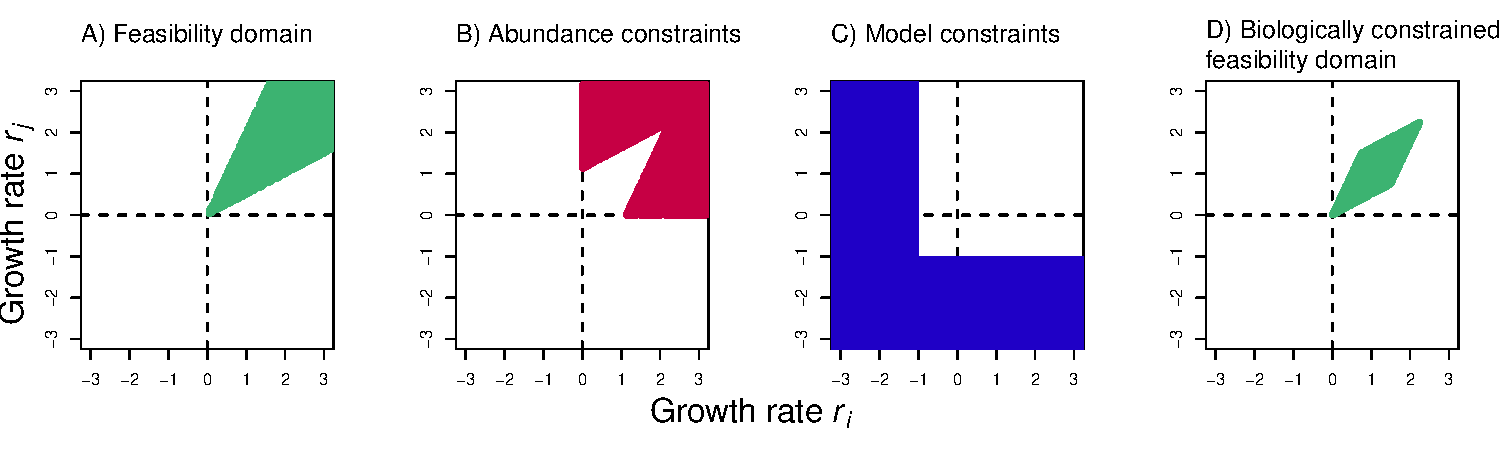
\includegraphics[width=1\textwidth]{figures/chapter3_fig1.pdf}}
  \caption[Estimation of the biologically-constrained feasibility domain]{Estimation of the biologically-constrained feasibility domain ($\beta$). A) We show the feasibility domain (green) given a hypothetical competition matrix with intraspecific competition coefficients equal to $1$ and interspecific competition coefficients equal to $0.5$. B) Part of the parameter space corresponds to species equilibrium abundances that are greater than specified abundance constraints (red). For simplicity, we used the same hypothetical abundance constraints for both species of $N^* \le 1.5$. C) Part of the the parameter space also falls outside model-based constraints (blue), assuming both species' density dependence is described by the Beverton--Holt model. D) The space of the feasibility domain that does not overlap with abundance or model-based constraints gives the biologically-constrained feasibility domain ($\beta$, green). }
  \label{fig:domain}
\end{figure}


\subsubsection*{Distance from the edge}

If two species' set of growth rates $r_{i}$ and $r_{j}$ are inside $\beta$, the two species are predicted to coexist. But there is more information contained in this comparison than a yes or no outcome. For example, the further those growth rates are from the edge of $\beta$, the less likely it is that perturbations to them will change the coexistence prediction. The minimum distance from the set of growth rates to the edge of $\beta$ is a measure of the susceptibility of qualitative coexistence predictions to perturbations of species' growth rates and interactions. We called this minimum distance $\delta$. To indicate when species growth rates are outside $\beta$, we multiplied $\delta$ by negative one. Large, positive values of $\delta$  thus imply species are confidently coexisting, large negative values imply species are confidently excluding each other, and values closer to zero imply small perturbations might change the predicted outcomes. We describe how exactly we quantify $\delta$ in Appendix B.


\subsubsection{Relative coexistence ratio}

As a basis of comparison, it is also convenient to quantify the parameter space that allows both species to grow in monoculture. Importantly, this parameter space can also be expressed as an area, and this area is also subject to abundance and model constraints. We called this area $\gamma$, and mathematical details of how to calculate the size of it can be found in S3 of the Supporting Information. By comparing the size of the parameter space where both species can coexist ($\beta$) to the size of the space where species can grow in monoculture ($\gamma$), we can quantify the importance of interspecific interactions relative to intraspecific interactions. This comparison can be expressed as a ratio $\rho$ that we call the relative coexistence ratio. If this ratio is equal to one, then species coexistence is as likely as species growing in monoculture; if this ratio is lower than one, then the parameter space where the two species can coexist is smaller than the parameter space where each species can grow in monoculture,  and it is less likely they can coexist when interacting; finally, ratios bigger than one imply that species facilitate each other, and it is more likely for them to coexist when interacting than to grow in monoculture. We show an example of how different values of $\beta$ and $\gamma$ determine the values of $\rho$, as well as their relationship to the distance from the edge $\delta$ in Fig.~\ref{fig:rho_delta}.

\subsubsection{An alternative model of density dependence}

%\subsection*{Alternative models for density dependence}

The Beverton--Holt model is only one of many phenomenological models used to describe density-dependent performance of annual plants. There is no general rule on how to choose the appropriate phenomenological model to describe the effect of species interactions, and it is often a choice governed by mathematical convenience \citep{mayfield2017higher}, the type of study system \citep{godwin2020empiricist}, and the governing paradigm around species interactions \citep{martyn2021identifying}. Indeed, there exists a plethora of related mathematical expressions that can quantify interactions between plants. One of them is the Ricker  model:
 \begin{equation}
 \label{Ricker}
   F_{i,t} = \lambda_{i} e^{(- \alpha_{ii}g_{i}N_{i,t} - \alpha_{ij}g_{j}N_{j,t})}\,,
\end{equation}
where the interpretation of the parameters remains the same as previously described \citep{ricker1954effects}. The Ricker model is known to be a biologically plausible and versatile model to quantify density dependence in annual plant communities, plus it has the virtue of being better able to capture both competitive and facilitative interactions \citep{mayfield2017higher,bimler_accurate_2018}.


\begin{figure}[H]
  \centerline{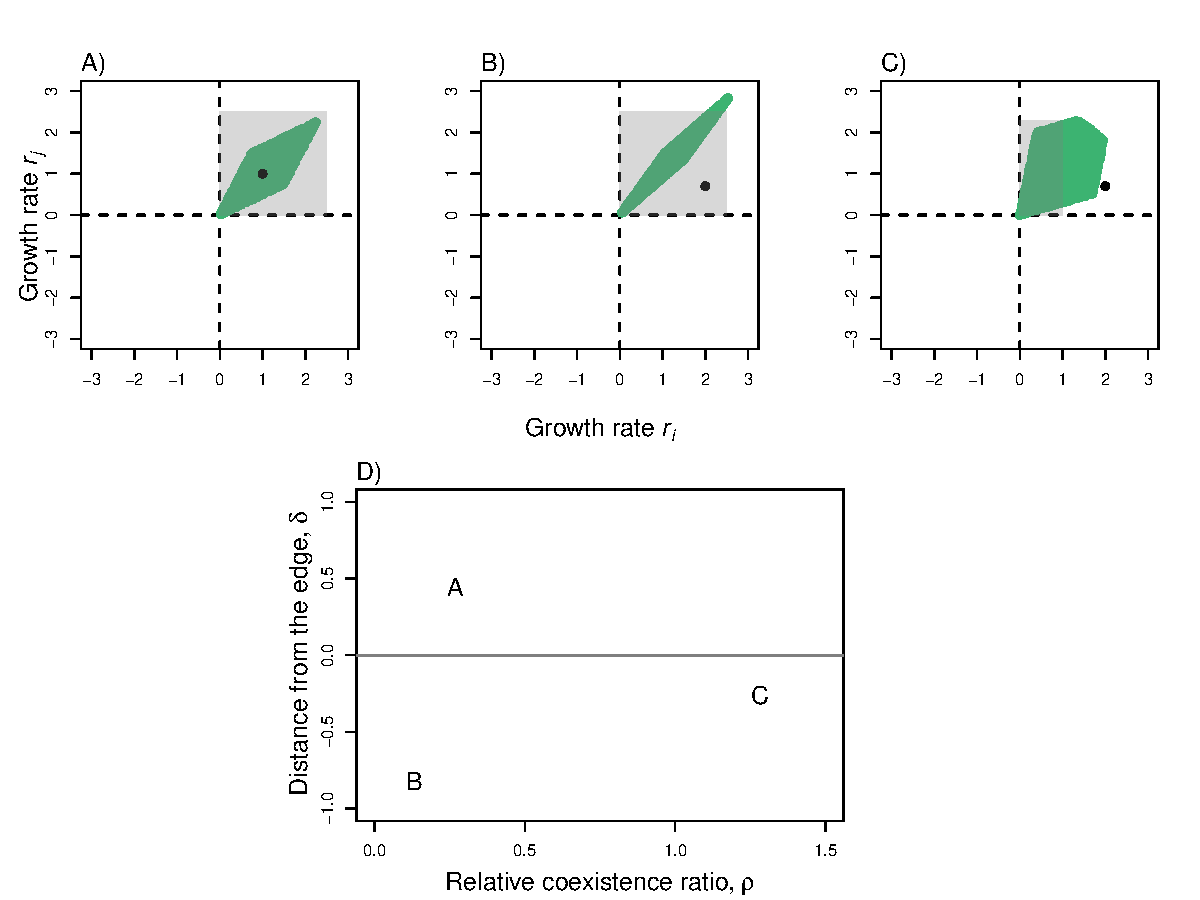
\includegraphics[width=1.1\textwidth]{figures/chapter3_fig2.pdf}}
  \caption[Examples of how different values of the biologically--constrained feasibility domain ($\beta$), the area in monoculture ($\gamma$), and species growth rates ($r_i$ and $r_j$) determine the values of the relative coexistence ratio ($\rho$) and the minimum distance from the edge ($\delta$).]{Examples of how different values of the biologically--constrained feasibility domain ($\beta$), the area in monoculture ($\gamma$), and species growth rates ($r_i$ and $r_j$) determine the values of the relative coexistence ratio ($\rho$) and the minimum distance from the edge ($\delta$). In A), B), and C) we show three hypothetical combinations of the biologically-constrained feasibility domain ($\beta$ in green), the parameter space where species can grow in monoculture ($\gamma$ in light grey), and a set of species growth rates (black circles). D) We show how the examples shown in A, B, and C correspond to different values of the relative coexistence ratio ($\rho$) and the distance from the edge ($\delta$).  }
  \label{fig:rho_delta}
\end{figure}


Similar to the process we followed from Eqns.~\ref{bh_equilibrium} to ~\ref{abundances}, the Ricker model has its own expression of growth rate at equilibrium. For species $i$, it is given by:
%\begin{equation}
%  r_{i} = 1 - \left(\frac{1-(1-g_{i})s_{i}}{g_{i}\lambda_{i}} \right).
%\end{equation}
%This expression necessarily implies that the model constraints on growth rates are different when using the Lotka--Volterra model than when using  the Beverton-Holt model: it has no lower limit but has an upper limit at one.
%In contrast, the composite growth rate for species $i$ in a Ricker model (Eqn.~\ref{Ricker}) is:
\begin{equation}
  r_{i}=\ln\left(\frac{g_{i}\lambda_{i}}{1-(1-g_{i})s_{i}}\right).
\end{equation}
This expression necessarily implies that the model constraints on growth rates are different when using the Ricker model than when using  the Beverton--Holt model: it has no model-based constraints on the lower and upper bounds of species growth rates. We summarize each of the models presented so far, their expressions of growth rates at equilibrium, and their lower and upper bounds in Table \ref{tab:definitions}


\begin{table}[h]

  \fontsize{10}{10}\selectfont
  \caption[Equilibrium growth rates and model constraints for the two models we used used to make coexistence predictions]{Equilibrium growth rates and model constraints for the two models we used used to make coexistence predictions. Growth rates are given by solving each model's equilibrium conditions in terms of seed densities. Upper and lower bounds are the result of how parameter bounds impact the values growth rate can take given the phenomenological model used to quantify density dependence.}
  \centering
  \label{tab:definitions}
 \begin{tabular*}{1\textwidth}{l @{\extracolsep{\fill}}lllll}
  \toprule
Model     & Growth rate & Lower bound& Upper bound \\\midrule
Beverton--Holt  &    $-1 + \left( \frac{g_{i}\lambda_{i}}{1-(1-g_{i})s_{i}} \right)$&  -1 &   Inf \\

%Lotka-Volterra  & $1 - \left(\frac{1-(1-g_{i})s_{i}}{g_{i}\lambda_{i}} \right)$          & -Inf &  1 \\
Ricker    & $\ln\left(\frac{g_{i}\lambda{i}}{1-(1-g_{i})s_{i}}\right)$  &   -Inf       &  Inf\\
\bottomrule
\end{tabular*}
\end{table}

\subsubsection*{Multi-model predictions of species coexistence}

By parameterizing a phenomenological model of plant competition, like the Beverton--Holt (Eqn.~\ref{Beverton-Holt}), we get a description of how seed set decreases with neighbor density. Perhaps more importantly, by linking this model to  Eqn.~\ref{annual_plant} we can make a prediction about whether or not two species are able to coexist. So far, we have been working with the implicit assumption that the same model describes the density dependence of the two species. However, there is no \textit{a priori} reason to assume this is the case, especially in an empirical case where different models can provide comparable fits \citep{hart2018quantify}.


To predict coexistence using a different density-dependence model per species, we still must solve for species equilibrium abundances as a function of growth rates and competition (Eqn.~\ref{abundances}). Unlike the single-model approach, each species' growth rate has its own formulation based on the model describing each species realized fecundity (Table \ref{tab:definitions}). As in the previous approach, if Eqn.~\ref{abundances} predicts positive abundances for both species within the bounds of each species' model and abundance constraints, species are predicted to coexist. Importantly, both $\beta$ and $\gamma$ become a function of four potential constraints: the set of lower and upper bounds per species. Having imposed those constraints, the relative coexistence ratio $\rho$ and the distance from the edge $\delta$ can again be calculated as described previously.


\subsection*{The interplay of different forms of uncertainty}

\subsubsection*{Data}

To assess the empirical relevance of different sources of uncertainty, we made coexistence predictions using parameter estimates inferred directly from a set of competition experiments. During 2017, we conducted pairwise competition experiments between two annual plants, \textit{Vellia rosea} and \textit{Trachymene cyanopetala}. Our experiments took place in the West Perenjori Nature Reserve in Western Australia (-29.479$^{\circ}$S, 116.199$^{\circ}$E). The reserve is dominated by York gum-jam woodlands, which support an understory of mixed native and exotic annual grasses and forbs \citep{dwyer2015climate}.

Using locally-collected seeds, we set up pairwise response--surface experiments. Response--surface experiments vary the densities of both species independently by using treatments with factorial combinations of the two species at two or more densities, and have the advantage of being able to accurately distinguish intra and interspecific competition \citep{inouye_response_2001, hart2018quantify}. To study how abiotic conditions change coexistence predictions, we conducted the experiments in two contrasting environments: a \textit{woody} environment, where plants interacted within 30 cm of woody debris, and a \textit{open} environment, where plants interacted at least 1 m outside the woody debris.

To implement our response--surface experiments, in October 2017 we first weeded out aboveground biomass of plants inside of circular plots with a 7.5 cm radius. This neighborhood radius is sufficiently large to capture local plant--plant interactions within the study system \citep{martyn2021identifying}. Each plot was then sown at different densities of each species as a focal: an invasion density where only one individual was sown, low density (15 seeds in total), medium density (30 seeds in total), and high density (60 seeds in total). In each plot, we also varied the densities with which the non-focal species was sown: either absent, medium or high. Treatments therefore consisted of combinations of the density of each species sown as a focal, the density of each species sown as a competitor, and the environment where interactions took place. We had four replicates per treatment, which yielded 256 plots in total. Plants germinated, and we thinned plots in composition in July 2018 (i.e., we weeded out neighbors that were not originally sowed). We collected the seeds produced after the growing season in October 2018 and also counted the number of conspecifics plant individuals ($n_{i}$), heterospecifics ($n_{j}$), and other neighbors ( $n_{k}$ i.e., plants that germinated after the plots were thinned in composition) in the plot at the time of seed collection.

Finally, we relied on a different set of data to obtain estimates of the survival and germination rates of each of our focal species in the field \citep{towers2021variable}, as well as the maximum abundance each species could achieve in the neighborhood radius where interactions took place. We show these values of seed survival rate, germination rate, and maximum abundance per species in Appendix B.

\subsubsection*{Statistical inference}

We fit Eqns.~\ref{Beverton-Holt} and~\ref{Ricker} separately for both of our focal species in order to get the relevant parameter estimates necessary to make coexistence predictions. For both species, we fit these non-linear models with a Bayesian framework using Hamiltonian Monte Carlo (HMC) methods. We used Bayesian inference to explicitly incorporate the uncertainty surrounding model parameters in probability distributions \citep{mcelreath_statistical_2018}. Across all models, we explicitly accounted for the environment where seeds were sown in our parameter estimates. For all of the parameters across all models, we did this by allowing the \textit{woody} environment to act as a dummy variable, $W$, that indicates the change in the environmental condition. For example, the fecundity in the absence of competition for species $i$ while in the \textit{woody} environment would be given by $\lambda_{i} + \lambda_{i,w}W$, where parameters with the subscript $w$ quantify the change due to the \textit{woody} environment.


For all models and all environmental conditions, we constrained the fecundity in the absence of competition  to be positive in order to keep our predictions biologically plausible. However, we did not constrain interaction parameters to be positive, allowing them to capture both competitive and facilitative interactions. Across all model fits, we included an extra term ($\alpha_{ik}$) to account for the effect of unidentified species in the experiment ($n_{k}$). We fit this extra interaction term to improve the parameter estimates  related to our focal species, but because we do not know their other parameters we could not model coexistence outcomes with these other neighbors.

We assumed the response variable, seeds produced per focal individual, followed a Poisson distribution for both species. Consequently we fit our non-linear models using the Poisson family and the identity link. We used the same weakly informative priors for the parameters in the Beverton--Holt model (Eqn.~\ref{Beverton-Holt}) and the Ricker model (Eqn.~\ref{Ricker}). As an example, the full description of the Beverton--Holt model for species $i$ is:

\begin{align}
 F_{i} \sim& {\textrm{Poisson}}(\rho_{i}) && \\
\rho_{i} =& \frac{e^{\lambda_{i} + \lambda_{i,w}W}} {1 + (\alpha_{ii} + \alpha_{ii,w}W)n_{i} + (\alpha_{ij} + \alpha_{ij,w}W) n_{j} + (\alpha_{ik} + \alpha_{ik,w}W)n_{k}} &&   \\
{ \left \{ \lambda_{i}, \lambda_{i,w} \right \}} \sim& {\textrm{Normal}}(0,1) &&\\
 { \left \{ \alpha_{ii}, \alpha_{ii,w} \right \}} \sim& {\textrm{Normal}}(0,1) &&\\
 {\left \{ \alpha_{ij}, \alpha_{ij,w} \right \}} \sim& {\textrm{Normal}}(0,1) &&\\
 {\left \{ \alpha_{ik}, \alpha_{ik,w} \right \}} \sim& {\textrm{Normal}}(0,1) &&
\end{align}
